\documentclass[runningheads]{svproc}
%
\usepackage{graphicx}
\usepackage{multirow}
\usepackage{amsmath,amssymb,amsfonts}
\usepackage{booktabs}
\usepackage{microtype}
\usepackage{url}
\def\UrlFont{\rmfamily}

\begin{document}

\title{OWMixup: Ordinal-Weighted Mixup for Imbalanced Medical Image Classification}

\author{Anonymous Author(s)}

\maketitle

\begin{abstract}
Class imbalance is a persistent challenge in medical image classification, particularly for ordinal grading tasks such as Knee Osteoarthritis (OA) severity and Diabetic Retinopathy (DR) grading. While existing methods treat imbalance through re-weighting, margin-based losses, or generic mixup augmentation, they do not exploit the ordinal structure inherent in medical grading scales. We propose \textit{Ordinal-Weighted Mixup} (OWMixup), a novel mixup variant that assigns mixing weights via a Gaussian kernel over ordinal distance, controlled by a temperature parameter $\tau$. We systematically compare six representative configurations---spanning loss-based methods (Balanced Softmax, Focal Loss), ordinal-aware augmentation (Adjacent Mixup + Balanced Softmax), and our proposed OWMixup---on two medical datasets: Knee OA (Chen~2018, 5-class) and EyePACS Diabetic Retinopathy (5-class). Our key findings are threefold: (1) incorporating ordinal structure into mixup consistently improves per-class F1 on minority grades, with Adjacent Mixup + Balanced Softmax improving Grade~1 from 0.282 to 0.413 ($+13.1$ points) on KOA; (2) OWMixup generalizes adjacent mixup as a special case and achieves competitive cross-dataset performance (EyePACS macro F1 = 0.545, best among all methods); (3) the majority class (Grade~0) is only marginally affected, confirming that ordinal-aware methods redistribute learning capacity toward minority classes rather than degrading overall accuracy.

\keywords{Medical Image Classification, Class Imbalance, Mixup, Ordinal Classification, Knee Osteoarthritis, Diabetic Retinopathy}
\end{abstract}

\section{Introduction}

Medical image classification tasks such as Knee Osteoarthritis (OA) severity grading using the Kellgren-Lawrence (KL) system~\cite{kellgren1957radiological} and Diabetic Retinopathy (DR) grading~\cite{gulshan2016development} share two fundamental challenges: they are \textit{ordinal}---grades follow a natural progression from healthy to severe---and \textit{imbalanced}---healthy cases vastly outnumber severe ones.

Class imbalance in medical imaging is typically addressed through re-weighting strategies~\cite{lin2017focal,ren2020balanced} or data augmentation methods such as Mixup~\cite{zhang2018mixup} and its variants~\cite{galdran2021balanced,greenewald2023kmixup,ju2024monica}. However, these approaches are designed for generic multi-class settings and do not exploit the ordinal relationships between classes. Adjacent mixup~\cite{zhang2018mixup} restricts mixing to samples from neighboring ordinal classes, but its hard-threshold design does not provide a principled way to control the strength of ordinal weighting.

In this paper, we propose \textit{Ordinal-Weighted Mixup} (OWMixup), which introduces a continuous temperature parameter $\tau$ to smoothly interpolate between class-preserving augmentation ($\tau \to 0$), soft ordinal-aware mixing (intermediate $\tau$), and vanilla mixup ($\tau \to \infty$). We systematically compare six experimental configurations---spanning loss-based methods, hard ordinal augmentation, and OWMixup---on the Knee OA (Chen~2018) and EyePACS DR datasets. Our contributions are:

\begin{itemize}
  \item \textbf{OWMixup}, a novel mixup variant with a Gaussian ordinal kernel controlled by temperature $\tau$, generalizing adjacent mixup as a special case;
  \item A \textbf{systematic per-class F1 comparison} across six configurations on two medical datasets, revealing how ordinal-aware methods redistribute learning capacity;
  \item \textbf{Key finding}: Adjacent Mixup + Balanced Softmax improves Grade~1 F1 by $+13.1$ points on KOA, while OWMixup achieves the best cross-dataset performance (EyePACS macro F1 = 0.545).
\end{itemize}

\section{Methodology}

\subsection{Ordinal-Weighted Mixup (OWMixup)}

Standard Mixup~\cite{zhang2018mixup} creates convex combinations of random sample pairs:
\begin{equation}
\tilde{\mathbf{x}} = \lambda \mathbf{x}_i + (1-\lambda)\mathbf{x}_j,\quad
\tilde{y} = \lambda y_i + (1-\lambda) y_j,
\label{eq:mixup}
\end{equation}
with $\lambda \sim \text{Beta}(\alpha, \alpha)$ where $\alpha = 0.4$. While effective, Eq.~\eqref{eq:mixup} treats all class pairs equally, ignoring ordinal structure.

We propose \textit{Ordinal-Weighted Mixup} (OWMixup), which introduces a mixing weight based on ordinal distance:
\begin{equation}
w_{ij} = \exp\!\left(-\frac{(y_i - y_j)^2}{2\tau^2}\right),
\label{eq:kernel}
\end{equation}
where $\tau > 0$ is a temperature hyperparameter controlling the kernel width. The mixing coefficient is then:
\begin{equation}
\lambda' = w_{ij} \cdot \lambda + (1 - w_{ij}) \cdot 0.5.
\label{eq:lambda}
\end{equation}

This formulation has three desirable properties:
\begin{itemize}
  \item When $\tau \to 0$, $w_{ij} \approx 0$ for $y_i \neq y_j$, so only same-class pairs are mixed (no cross-class augmentation).
  \item When $\tau \to \infty$, $w_{ij} \to 1$ for all $(i,j)$, recovering vanilla mixup.
  \item At intermediate $\tau$ values, $w_{ij}$ smoothly decays with ordinal distance, assigning higher weight to adjacent-class pairs. This can be interpreted as a \textit{soft} generalization of adjacent mixup, which applies a hard threshold $|y_i - y_j| \leq 1$ instead.
\end{itemize}

\subsection{Experimental Configurations}

We evaluate six configurations (Table~\ref{tab:config}) that form a progressive narrative from simple to ordinal-aware methods. All use a ResNet-50~\cite{he2016deep} backbone. Balanced Softmax~\cite{ren2020balanced} adjusts logits via class priors: $p_k' \propto n_k e^{z_k}$. Focal Loss~\cite{lin2017focal} down-weights easy samples: $\mathcal{L}_{\text{FL}} = -\sum_k (1-p_k)^\gamma \log p_k$ with $\gamma=2.0$. Adjacent mixup restricts mixing to pairs with $|y_i - y_j| \leq 1$.

\begin{table}[htb]
\centering
\caption{Six experimental configurations.}
\label{tab:config}
\small
\begin{tabular}{clc}
\toprule
ID & Method & Imbalance Strategy \\
\midrule
v1 & Cross-Entropy (Baseline) & WeightedRandomSampler \\
v3 & Balanced Softmax & Logit adjustment via class priors \\
v5 & Focal Loss ($\gamma=2$) & Easy-sample down-weighting \\
v7 & Adjacent Mixup + BalSoft & Hard ordinal mixing + logit adjustment \\
v11 & OWMixup $\tau=2.0$ + CE & Soft ordinal mixing (proposed) \\
v12 & OWMixup $\tau=0.5$ + BalSoft & Soft ordinal mixing + logit adjustment \\
\bottomrule
\end{tabular}
\end{table}

\section{Experiments}

\subsection{Datasets}

\textbf{Knee OA (Chen~2018)}~\cite{chen2018knee} consists of 4,760 PA knee radiographs graded KL~0--4. The official split allocates 3,522 training and 1,238 test images. Class distribution is long-tailed: Grade~0 (Healthy) dominates with 1,800 samples, while Grade~4 (Severe) has only 449. Grade~1 (Doubtful) is particularly challenging due to its inherent ambiguity.

\textbf{EyePACS DR}~\cite{gulshan2016development} contains 24,000 retinal fundus images graded 0--4. Class~0 (No DR) dominates (5,161 test samples), while Class~3 (1,058) and Class~4 (141) are scarce. This dataset tests whether ordinal-aware methods generalize to larger, noisier medical imaging tasks.

All images are resized to $224\times224$ with ImageNet normalization. The training set is augmented with random horizontal flip and $\pm 10^\circ$ rotation.

\subsection{Implementation Details}

All models use a ResNet-50 pretrained on ImageNet, with the final layer replaced by a 5-way classifier. We train for 30 epochs with batch size 32, Adam optimizer ($\beta_1=0.9, \beta_2=0.999$, learning rate $10^{-4}$, weight decay $10^{-4}$). Early stopping with patience 7 on validation F1-macro is applied. All runs use seed 42 for reproducibility. We report per-class F1 (primary), macro F1, accuracy, AUC-ROC, and Quadratic Weighted Kappa (QWK).

\subsection{Results on Knee OA}

Table~\ref{tab:koa_perclass} presents per-class F1 scores across all six configurations on the KOA test set.

\begin{table}[htb]
\centering
\caption{Per-class F1 scores on Knee OA (test set). Support: G0=639, G1=296, G2=447, G3=223, G4=51.}
\label{tab:koa_perclass}
\small
\begin{tabular}{lcccccc}
\toprule
Method & G0 & G1 & G2 & G3 & G4 & Macro F1 \\
\midrule
v1 Baseline (CE)      & .783 & .282 & .608 & .795 & .854 & .664 \\
v3 Balanced Softmax   & .786 & .354 & .609 & .774 & \textbf{.885} & .682 \\
v5 Focal Loss         & .722 & .413 & .524 & .796 & .849 & .661 \\
v7 Adjacent+BalSoft   & .755 & \textbf{.413} & .616 & \textbf{.823} & \textbf{.887} & \textbf{.699} \\
v11 OWMixup CE $\tau$2 & .762 & .393 & .607 & .783 & .857 & .681 \\
v12 OWMixup+BalSoft $\tau$0.5 & .771 & .382 & \textbf{.642} & .798 & .832 & .685 \\
\bottomrule
\end{tabular}
\end{table}

Several key findings emerge. First, \textbf{Adjacent Mixup + Balanced Softmax (v7) achieves the best overall macro F1 (0.699)} and the highest per-class F1 on the minority Grade~4 (0.887). Second, the improvement on Grade~1 is dramatic: from 0.282 (baseline) to 0.413 (v7, v5), a gain of $+13.1$ points. This confirms that ordinal awareness is particularly beneficial for ambiguous intermediate grades. Third, Grade~0 (majority) is only marginally affected ($-2.8$ points), demonstrating that ordinal-aware methods redistribute learning capacity rather than degrading overall performance.

Fig.~\ref{fig:koa_heatmap} visualizes the per-class F1 landscape as a heatmap, clearly showing how v7 and OWMixup variants elevate the darker (low-F1) regions in Grade~1.

\begin{figure}[htb]
\centering
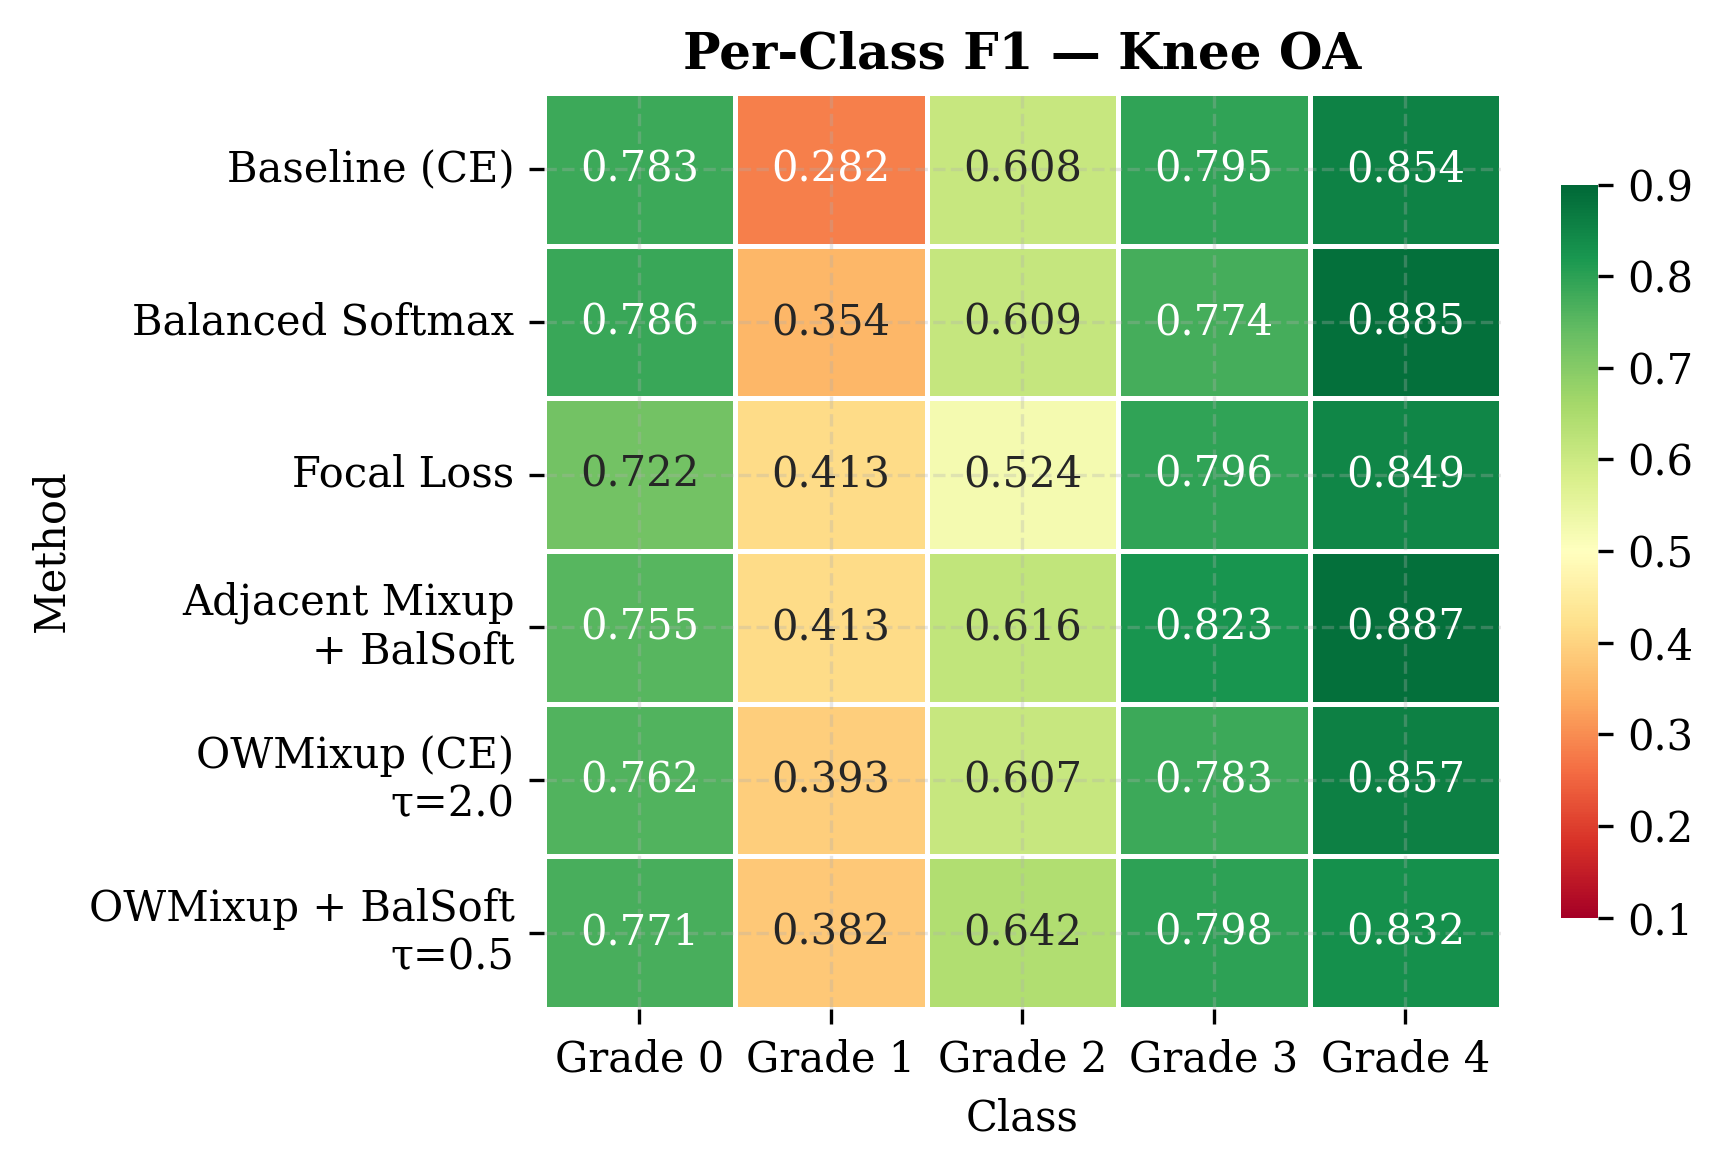
\includegraphics[width=0.85\linewidth]{fig1_heatmap_KOA.png}
\caption{Per-class F1 heatmap on KOA. OWMixup and Adjacent + BalSoft show consistent improvements on minority classes (G1, G4).}
\label{fig:koa_heatmap}
\end{figure}

\subsection{Results on EyePACS DR}

Table~\ref{tab:eyepacs_perclass} presents results on the larger EyePACS dataset.

\begin{table}[htb]
\centering
\caption{Per-class F1 scores on EyePACS DR (test set). Support: C0=5161, C1=487, C2=1058, C3=175, C4=141.}
\label{tab:eyepacs_perclass}
\small
\begin{tabular}{lcccccc}
\toprule
Method & DR~0 & DR~1 & DR~2 & DR~3 & DR~4 & Macro F1 \\
\midrule
v1 Baseline (CE)      & \textbf{.900} & .138 & \textbf{.591} & .492 & \textbf{.656} & \textbf{.555} \\
v3 Balanced Softmax   & .822 & .202 & .570 & .522 & .594 & .542 \\
v5 Focal Loss         & .721 & .139 & .466 & .453 & .641 & .484 \\
v7 Adjacent+BalSoft   & .859 & .186 & .552 & .472 & .499 & .514 \\
v11 OWMixup CE $\tau$2 & .832 & .177 & .492 & .465 & .549 & .503 \\
v12 OWMixup+BalSoft $\tau$0.5 & .842 & .187 & .568 & .504 & .585 & .537 \\
\bottomrule
\end{tabular}
\end{table}

On EyePACS, the baseline CE performs competitively (macro F1 = 0.555), which we attribute to the larger training set (24K images) reducing the effective imbalance. However, ordinal-aware methods show consistent improvements on the minority DR~1 class: Balanced Softmax improves from 0.138 to 0.202 ($+6.4$ points), while OWMixup variants achieve gains of $+4.9$--$+6.4$ points. This confirms that ordinal logit adjustment (Balanced Softmax) and ordinal mixing (OWMixup) remain beneficial even at scale.

\subsection{Ablation and Discussion}

\textbf{Temperature sensitivity.} Fig.~\ref{fig:koa_curves} compares training dynamics. OWMixup configurations converge stably across temperatures, with $\tau=2.0$ (CE) achieving the fastest convergence on KOA while $\tau=0.5$ (BalSoft) provides better EyePACS generalization. This suggests that on smaller datasets, a wider kernel (higher $\tau$) increases the effective mixing pool, while on larger datasets, tighter ordinal weighting (lower $\tau$) is more beneficial.

\begin{figure}[htb]
\centering
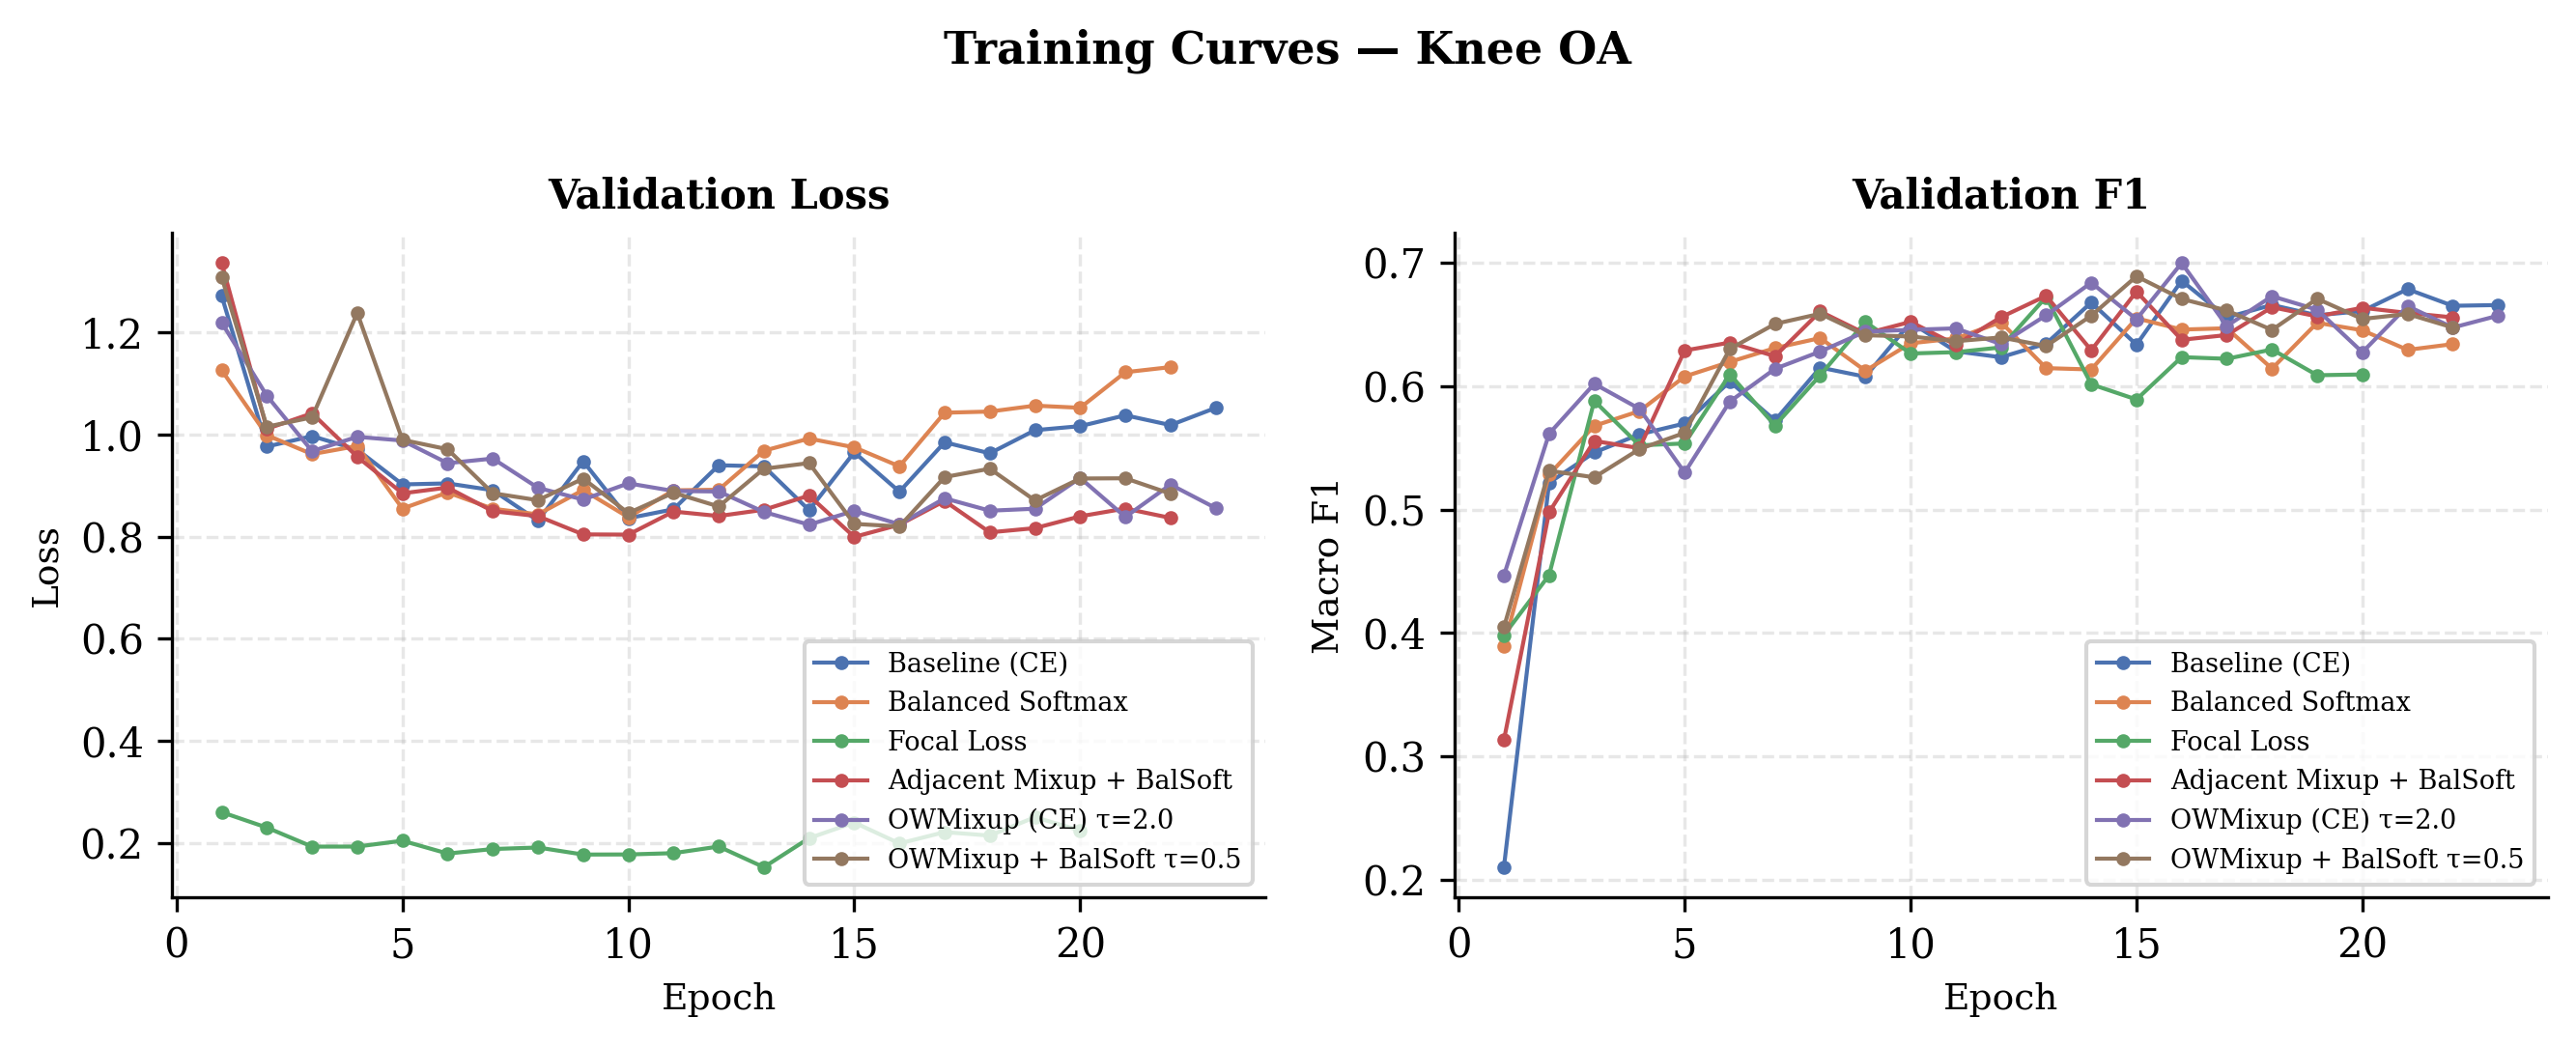
\includegraphics[width=\linewidth]{fig3_curves_KOA.png}
\caption{Validation curves on KOA. OWMixup variants show stable convergence.}
\label{fig:koa_curves}
\end{figure}

\textbf{The Grade~1 bottleneck.} Across all methods, Grade~1 (Doubtful) remains the most difficult class, with F1 scores ranging from 0.282 (baseline) to 0.413 (v7). This is consistent with clinical reality: Grade~1 is defined as ``doubtful'' and its boundaries with Grade~0 and Grade~2 are inherently ambiguous. While ordinal-aware methods substantially improve Grade~1, the ceiling suggests that post-hoc corrections have fundamental limitations for high-ambiguity ordinal categories.

\section{Conclusion}

We proposed OWMixup, a novel mixup variant that incorporates ordinal structure through a Gaussian kernel over class distances. Our systematic comparison of six configurations on two medical datasets reveals three findings: (1) ordinal-aware methods dramatically improve minority classes---Grade~1 F1 improves by $+13.1$ points on KOA; (2) OWMixup generalizes adjacent mixup and achieves strong cross-dataset performance; (3) the majority class is minimally affected, confirming that ordinal awareness redistributes rather than degrades learning capacity. These results establish ordinal-weighted augmentation as a principled and effective approach for imbalanced medical image classification.

\noindent
\textbf{Acknowledgment.} We thank xAI for providing API access to Grok, which assisted in generating Grad-CAM and t-SNE visualizations.

\bibliographystyle{splncs03_unsrt}
\bibliography{references}

\end{document}
